\documentclass{article}
\usepackage{tikz}
\usepackage{tikz-qtree}
\usepackage{amsmath}
\usepackage{amssymb}
\begin{document}
\section*{Ordered Trees}


Given an ordered tree T, Let O be the first node in a preorder traversal of T that is not in the left-down path of T. Let P be O's parent, and let L be P's leftmost child (or, equivalently, O's left sibling).  The tree below gives an example illustrating these three nodes. 

$D=[1, 1, 1, 1, 1, 1, 0, 0, 0, 0, 1, 1, 0, 0, 1, 0, 0, 1, 1, 0, 0, 0]$

$T=$

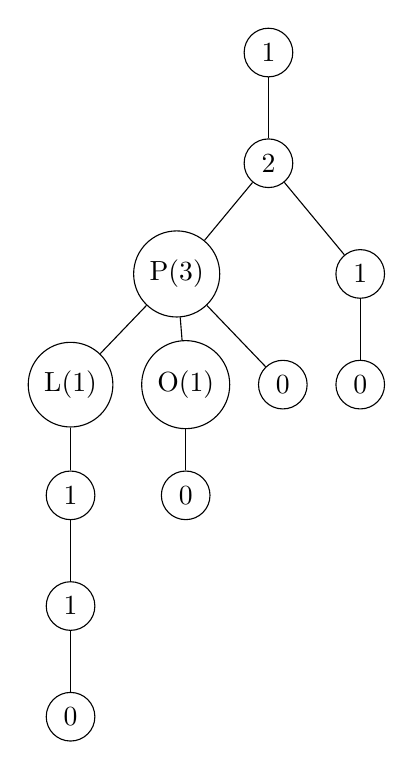
\begin{tikzpicture}[every tree node/.style={draw,circle},sibling distance=10pt, level distance=40pt]
\tikzset{edge from parent/.style={draw, edge from parent path=
    {(\tikzparentnode) -- (\tikzchildnode)}}}
    \Tree [.1 [.2 [.P(3) [.L(1) [.1 [.1 [.0 ] ] ] ] [.O(1) [.0 ] ] [.0 ] ] [.1 [.0 ] ] ] ]
\end{tikzpicture}

\noindent Let D be the dyck word corresponding to T and let k be the index of the first 01 prefix in D. Note that the node O within T corresponds to $D_k$.

\noindent The cool-lex rule for shifts in ordered trees can be broken down into 3 cases:
\begin{itemize}
    \item Case 1: O has at least 1 child
	
	This case corresponds to the case where $D_{k+1}=1$
	
	Shift L to be O's first child. 


    \item Case 2: O has no children and O is the child of the root

	This case corresponds to the case where $D_{k+1}=0$ and the non-increasing prefix is tight (i.e., the non-increasing prefix hsa exactly as many ones as zeroes).
	
	Shifts in this case are the same as in case 1. 
	% \begin{itemize}
	%     \item test
	% \end{itemize}
    \item Case 3: O has no children and O is not child of the root

	This case corresponds to the case where $D_{k+1}=0$ and the non-increasing prefix is not-tight (i.e., the non-increasing prefix has more ones than zeroes). 

	Shift L to be the first child of P's parent

	Shift O to be the first child of the root. 

	Note: The order of these shifts matters. P cannot be the root, but if P's parent is the root, the O and L are both shifted to be P's first child. The shifting of O must be done second so that after both shifts are done O is the first child of the root. 


\end{itemize}


 Illustration of case 1 (shifting a 1): 

\bigskip

[1, 1, 1, 1, 1, 1, 0, 0, 0, 0, 1, 1, 0, 0, 1, 0, 0, 1, 1, 0, 0, 0] $\implies$

[1, 1, 1, 1, 1, 1, 1, 0, 0, 0, 0, 1, 0, 0, 1, 0, 0, 1, 1, 0, 0, 0]

\bigskip


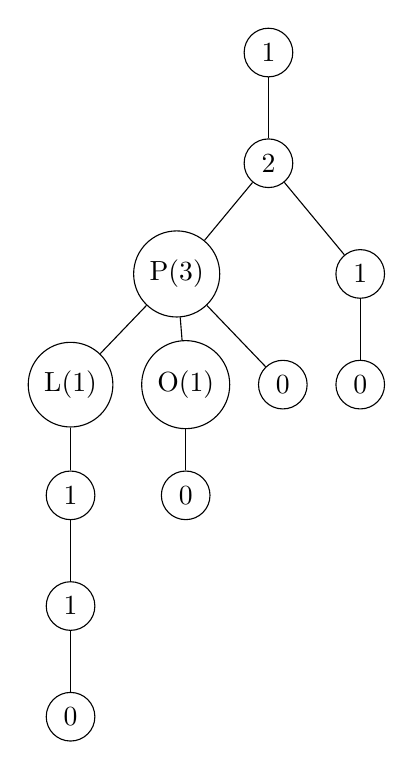
\begin{tikzpicture}[every tree node/.style={draw,circle},sibling distance=10pt, level distance=40pt]
\tikzset{edge from parent/.style={draw, edge from parent path=
    {(\tikzparentnode) -- (\tikzchildnode)}}}
    \Tree [.1 [.2 [.P(3) [.L(1) [.1 [.1 [.0 ] ] ] ] [.O(1) [.0 ] ] [.0 ] ] [.1 [.0 ] ] ] ]
\end{tikzpicture} $\implies$
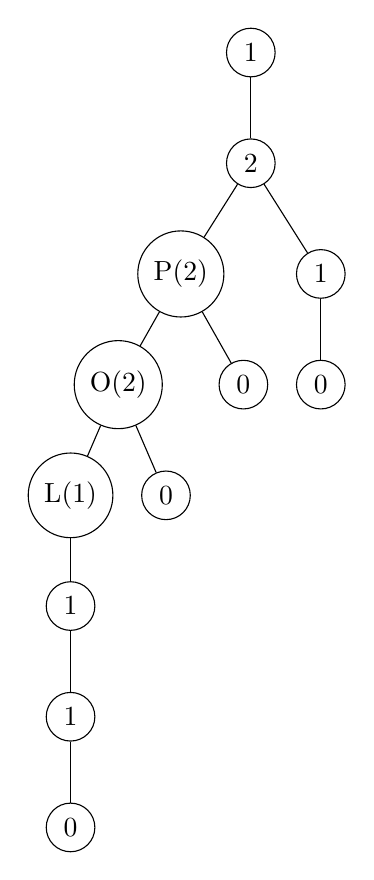
\begin{tikzpicture}[every tree node/.style={draw,circle},sibling distance=10pt, level distance=40pt]
\tikzset{edge from parent/.style={draw, edge from parent path=
    {(\tikzparentnode) -- (\tikzchildnode)}}}
    \Tree [.1 [.2 [.P(2) [.O(2) [.L(1) [.1 [.1 [.0 ] ] ] ] [.0 ] ] [.0 ] ] [.1 [.0 ] ] ] ]
\end{tikzpicture}


\pagebreak
Illustration of case 3 (shifting a 0): 
\bigskip

[1, 1, 1, 1, 1, 1, 1, 0, 0, 0, 0, 1, 0, 0, 1, 0, 0, 1, 1, 0, 0, 0]
$\implies$

[1, 0, 1, 1, 1, 1, 1, 1, 0, 0, 0, 0, 1, 0, 1, 0, 0, 1, 1, 0, 0, 0]

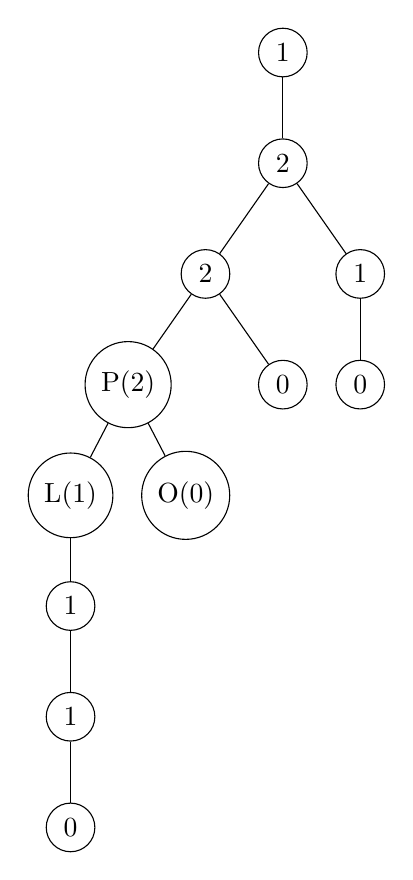
\begin{tikzpicture}[every tree node/.style={draw,circle},sibling distance=10pt, level distance=40pt]
\tikzset{edge from parent/.style={draw, edge from parent path=
    {(\tikzparentnode) -- (\tikzchildnode)}}}
    \Tree [.1 [.2 [.2 [.P(2) [.L(1) [.1 [.1 [.0 ] ] ] ] [.O(0) ] ] [.0 ] ] [.1 [.0 ] ] ] ]
\end{tikzpicture} $\implies$
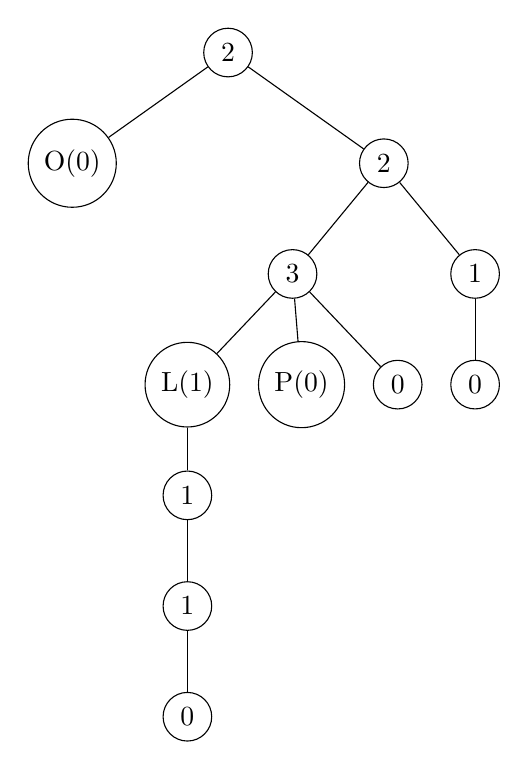
\begin{tikzpicture}[every tree node/.style={draw,circle},sibling distance=10pt, level distance=40pt]
\tikzset{edge from parent/.style={draw, edge from parent path=
    {(\tikzparentnode) -- (\tikzchildnode)}}}
    \Tree [.2 [.O(0) ] [.2 [.3 [.L(1) [.1 [.1 [.0 ] ] ] ] [.P(0) ] [.0 ] ] [.1 [.0 ] ] ] ]
\end{tikzpicture}

\pagebreak

Illustration of case 2 ($D_k=0$, prefix is tight, shift a 1)


\bigskip

[1, 1, 1, 0, 0, 0, 1, 0, 1, 0, 1, 0] $\implies$


[1, 1, 1, 1, 0, 0, 0, 0, 1, 0, 1, 0]


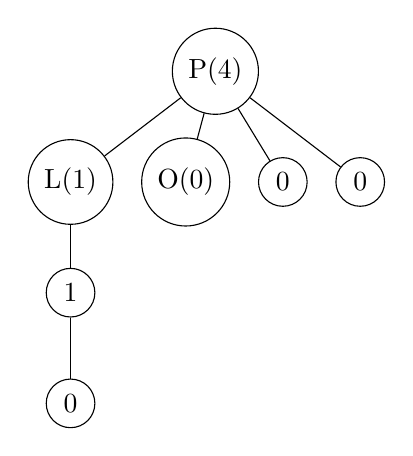
\begin{tikzpicture}[every tree node/.style={draw,circle},sibling distance=10pt, level distance=40pt]
\tikzset{edge from parent/.style={draw, edge from parent path=
    {(\tikzparentnode) -- (\tikzchildnode)}}}
    \Tree [.P(4) [.L(1) [.1 [.0 ] ] ] [.O(0) ] [.0 ] [.0 ] ]
\end{tikzpicture}  $\Longrightarrow$
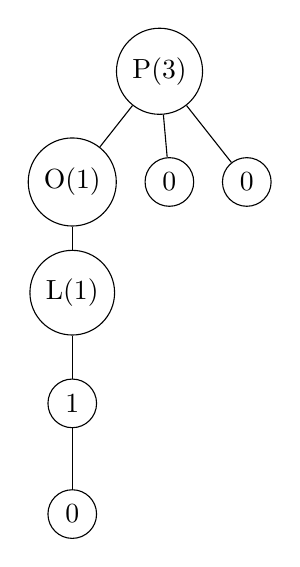
\begin{tikzpicture}[every tree node/.style={draw,circle},sibling distance=10pt, level distance=40pt]
\tikzset{edge from parent/.style={draw, edge from parent path=
    {(\tikzparentnode) -- (\tikzchildnode)}}}
    \Tree [.P(3) [.O(1) [.L(1) [.1 [.0 ] ] ] ] [.0 ] [.0 ] ]
\end{tikzpicture}

\end{document}
